\chapter{Where the cost of index calculus lives}\label{ch:model}

The cost of one index-calculus solve is a sum of terms. This chapter writes
them out, maps each lever of the programme to the term it acts on, gives
the measured cost of the operations the terms are counted in, and reports
which term dominates on every leaderboard row.

\section{The pipeline}

Fix a factor base $\Fb\subset E(\FF_q)$ of size $N$. A \emph{relation} is a
decomposition $aG+bQ=P_1+\cdots+P_m$ with every $P_i\in\pm\Fb$. Once about
$N$ independent relations are known, linear algebra over $\ZZ/r$ yields
$\log_G Q$. A heuristic count is enough to place the levers. A uniformly
random point decomposes into $m$ base points with probability about
$N^m/(m!\,r)$. Collecting $N$ relations therefore needs about
$m!\,r/N^{m-1}$ trials. The cold cost of one target is then
\begin{equation}\label{eq:cost}
  T \;\approx\;
  \underbrace{T_{\mathrm{setup}}(N)}_{\text{base, tables}}
  \;+\;
  \underbrace{\frac{m!\,r}{N^{m-1}}\;\frac{1}{\rho_{\mathrm{yield}}}\;
  C_{\mathrm{dec}}(N,m)}_{\text{relation collection}}
  \;+\;
  \underbrace{T_{\mathrm{LA}}(N,m)}_{\text{linear algebra}}
  \;+\;
  \underbrace{T_{\mathrm{target}}}_{\text{descent, check}}.
\end{equation}
Here $C_{\mathrm{dec}}$ is the cost of one decomposition attempt (the
\emph{oracle}). The factor $\rho_{\mathrm{yield}}\ge1$ collects everything
that makes a trial more productive than the heuristic: free relations,
large primes, symmetry, re-randomised targets. $T_{\mathrm{LA}}$ is roughly
$mN^2$ for sparse elimination. With rho's cost $\sqrt{\pi r/(2A)}$ on the
other side, the classical balance at $m=2$ with a constant-cost oracle gives
$N\approx r^{1/3}$ and $T\approx r^{2/3}$. That is why two-summand
prime-field index calculus loses ground to rho as $r^{1/6}$
(Chapter~\ref{ch:distance}). The $k$-sum oracle, a generic table of
signed $k$-sums, moves the exponent to $k/(2k-1)$, and no generic
single-target arm whose base logarithms are unknown can go below the collision floor of
Proposition~\ref{prop:collisionfloor}.

\section{The levers}

Table~\ref{tab:levers} lists, for each term of~\eqref{eq:cost}, the levers
the programme pulled and the sections that report them.

\begin{table}[t]
\centering\small
\begin{tabularx}{\linewidth}{@{}l>{\raggedright}X>{\raggedright\arraybackslash}p{3.0cm}@{}}
\toprule
Term & Levers pulled & Where \\
\midrule
$C_{\mathrm{dec}}$ & root finding of $S_3$; pair and meet-in-the-middle
  tables; $k$-sum tables; inherited F4, F5, F6-IC; gate-first order;
  harvest gates; $\FF_p$ F4; $D_4$ invariants; the Hilbert early stop on
  the weak-class cover & Ch.~\ref{sec:rootfinding}, \ref{sec:groebner},
  \ref{ch:extension}, \ref{ch:distance}; \S\ref{sec:pg-ksum}, \S\ref{sec:jac-jv} \\
$\rho_{\mathrm{yield}}$, $N$ & compact Frobenius orbits; free relations;
  stride-renewed targets; greedy coverage; $n=83$ base selection; double
  large primes; the Joux--Vitse sieve route & Ch.~\ref{sec:koblitz}, \ref{sec:prime}, \ref{sec:transfer}; \S\ref{sec:jac-jv} \\
$T_{\mathrm{setup}}$ & stacked producer; cache-blocked pair table; u64 root
  batching & Ch.~\ref{sec:koblitz}, \ref{sec:prime} \\
$T_{\mathrm{LA}}$ & CADO-style filter and Wiedemann; structured Gaussian
  elimination; block Wiedemann; first-dependency stop; post-Gröbner
  linear stage & Ch.~\ref{sec:koblitz}, \ref{sec:prime},
  Ch.~\ref{ch:extension}, \ref{sec:transfer}, \ref{ch:audit} \\
the exponent & genus-three transfer (cubic GHS); $k=4$ extension fields &
  Ch.~\ref{ch:extension}, \ref{sec:transfer} \\
fixed floor & none: the collision floor bounds every generic
  single-target arm with unknown base logarithms at $\ge1.5\times$ rho & \S\ref{sec:gf-collision} \\
\bottomrule
\end{tabularx}
\caption[]{The terms of~\eqref{eq:cost} and the levers that act on them.}
\label{tab:levers}
\end{table}

\section{Measured cost of one operation}\label{sec:model-opcost}

Every $S$ in this treatise is a count of group-addition equivalents (GAE).
Native work (lookups, row operations, square roots, Artin--Schreier solves,
word XORs) enters it through ratios pinned per instance in
\art{docs/ic/calibration.json}: nanoseconds per native operation over
nanoseconds per group addition, the median of three frozen boundary-ledger
runs on one Intel Xeon at 2.1\,GHz. Table~\ref{tab:fm-ledgerhost} gives the
absolute timings behind those ratios and Figure~\ref{fig:fm-opcost} plots
them. On that host a group addition costs 155--221\,ns on the prime
instances and 175--683\,ns on the binary and Koblitz instances; a doubling
costs $0.96$--$1.15$ additions on every instance (pinned ratios); a lookup
($2.4$--$4.5$\,ns), a row operation ($3.2$--$3.6$\,ns) and a word XOR
($0.46$--$0.51$\,ns) are flat in the field size. The ratios move by up to
$3.7$ between runs on one host, which is why they are pinned rather than
re-measured (\art{docs/ic/calibration.json}, field \texttt{why}).

\begin{table}[tbp]
\centering\scriptsize\setlength{\tabcolsep}{3.5pt}
% generated by make_tab_fm.py; do not edit
\begin{tabular}{@{}lrrrrrrrrr@{}}
\toprule
instance & $\log_2 r$ & add & double & inv. & sqrt & Legendre & lookup & row op & word XOR \\
\midrule
$\FF_p$, 10 bits & 9.7 & 213 & 204 & 93.3 & 64.4 & 48.1 & 2.59 & 3.53 & 0.48 \\
$\FF_p$, 12 bits & 11.9 & 155 & 175 & 108 & 77.7 & 65.8 & 2.65 & 3.60 & 0.50 \\
$\FF_p$, 14 bits & 14.0 & 164 & 185 & 124 & 109 & 81.0 & 2.53 & 3.46 & 0.49 \\
$\FF_p$, 16 bits & 16.0 & 177 & 204 & 137 & 1026 & 97.2 & 2.73 & 3.54 & 0.51 \\
$\FF_p$, 18 bits & 18.0 & 191 & 210 & 147 & 150 & 98.1 & 2.71 & 3.42 & 0.49 \\
$\FF_p$, 20 bits & 20.0 & 188 & 222 & 150 & 163 & 108 & 2.44 & 3.42 & 0.47 \\
$\FF_p$, 22 bits & 21.7 & 215 & 241 & 169 & 166 & 122 & 3.05 & 3.62 & 0.50 \\
$\FF_p$, 24 bits & 23.4 & 221 & 240 & 178 & 1020 & 125 & 3.02 & 3.46 & 0.49 \\
\midrule
instance & $\log_2 r$ & add & double & AS solve & Frobenius & $S_4$ pair & lookup & row op & word XOR \\
\midrule
random $\FF_{2^{15}}$ & 14.0 & 217 & 211 & 11.7 & 13.2 & 640 & 2.51 & 3.17 & 0.47 \\
random $\FF_{2^{18}}$ & 15.0 & 274 & 272 & 9.44 & 14.2 & 837 & 2.47 & 3.39 & 0.46 \\
random $\FF_{2^{21}}$ & 20.0 & 337 & 338 & 19.9 & 14.0 & 921 & 2.68 & 3.43 & 0.46 \\
random $\FF_{2^{24}}$ & 21.0 & 372 & 374 & 13.2 & 14.9 & 1053 & 2.60 & 3.58 & 0.49 \\
random $\FF_{2^{27}}$ & 24.4 & 421 & 456 & 32.1 & 16.2 & 1312 & 2.96 & 3.59 & 0.49 \\
K1 $\FF_{2^{11}}$ & 10.0 & 175 & 175 & 8.85 & 13.6 & -- & 2.58 & 3.48 & 0.49 \\
K0 $\FF_{2^{13}}$ & 11.0 & 202 & 208 & 10.3 & 13.7 & -- & 2.40 & 3.42 & 0.46 \\
K0 $\FF_{2^{15}}$ & 9.6 & 224 & 222 & 12.3 & 13.1 & 592 & 2.45 & 3.17 & 0.47 \\
K1 $\FF_{2^{17}}$ & 16.0 & 243 & 249 & 14.2 & 12.7 & -- & 2.58 & 3.29 & 0.47 \\
K1 $\FF_{2^{19}}$ & 18.0 & 301 & 302 & 17.3 & 14.3 & -- & 2.56 & 3.40 & 0.47 \\
K1 $\FF_{2^{23}}$ & 22.0 & 362 & 358 & 23.6 & 14.4 & -- & 3.18 & 3.33 & 0.48 \\
K1 $\FF_{2^{29}}$ & 15.4 & 468 & 478 & 35.0 & 15.5 & -- & 4.52 & 3.46 & 0.49 \\
K0 $\FF_{2^{31}}$ & 20.5 & 503 & 501 & 40.0 & 15.7 & 1482 & 3.72 & 3.53 & 0.48 \\
K0 $\FF_{2^{37}}$ & 27.8 & 627 & 610 & 53.1 & 16.3 & -- & 3.67 & 3.41 & 0.49 \\
K0 $\FF_{2^{39}}$ & 26.0 & 611 & 643 & 57.8 & 16.9 & -- & 3.67 & 3.41 & 0.48 \\
K0 $\FF_{2^{41}}$ & 39.0 & 683 & 677 & 65.2 & 17.1 & -- & 4.11 & 3.31 & 0.47 \\
\bottomrule
\end{tabular}

\caption[]{Nanoseconds per operation on the boundary ledger's host (Intel
Xeon, 2.1\,GHz, 4 logical cores), median of the three frozen runs
\art{docs/ic/runs/ic-boundary-ledger-round2-2026-09-21.json},
\art{docs/ic/runs/ic-boundary-ledger-round3-2026-09-21.json} and
\art{docs/ic/runs/ic-boundary-ledger-round3-rotation-2026-09-21.json}
(\texttt{ledger.instances[*].calibration}); medians computed by the
extraction recorded in \art{figures/data-fm-opcost.json}. ``inv.'' is a
field inversion, ``AS solve'' an Artin--Schreier solve, ``$S_4$ pair'' one
pair evaluation of the fourth summation polynomial. Prime square roots at
16 and 24 bits ($\approx1{,}020$\,ns) take the Tonelli--Shanks path. Shared
host, no isolation receipt: the timings are descriptive and enter $S$ only
as the pinned ratios. Table built by \art{figures/make_tab_fm.py}.}
\label{tab:fm-ledgerhost}
\end{table}

\begin{figure}[tbp]\centering
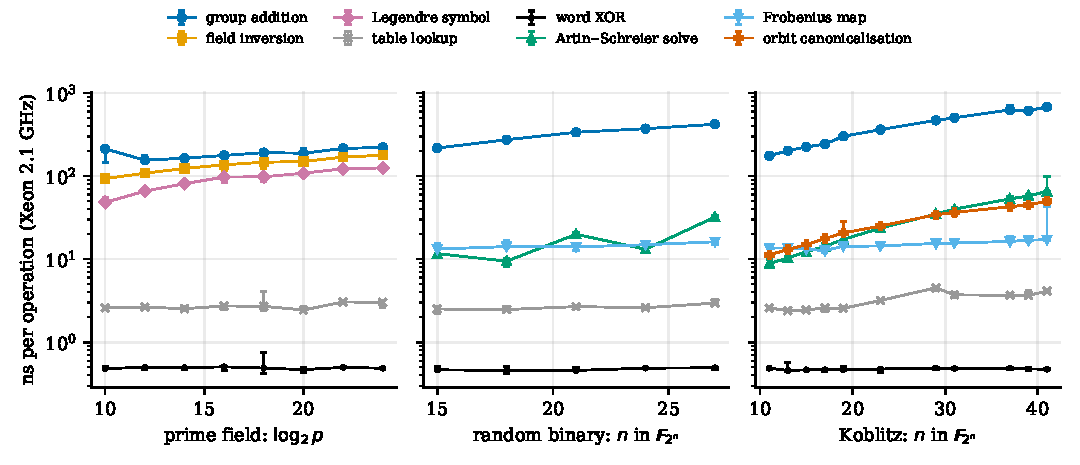
\includegraphics[width=\linewidth]{figures/fig-fm-opcost.pdf}
\caption[Nanoseconds per operation against field size]{Nanoseconds per operation against field size on the boundary
ledger's host, log scale; markers are medians of three frozen runs and bars
span their minimum and maximum. The group addition grows with the field;
lookups, row operations and word XORs do not, so their GAE price falls as
the field grows. Data: \art{figures/data-fm-opcost.json} (from
\art{docs/ic/runs/}); plot: \art{figures/make_fig_fm_opcost.py}.}
\label{fig:fm-opcost}
\end{figure}

Field arithmetic was measured separately. Table~\ref{tab:fm-fieldops}
collects the field multiplication, squaring and inversion costs on record.
On word-sized prime fields a Montgomery \texttt{u64} multiplication costs
about 10\,ns and an inversion 63 multiplications, or $1.69$ when $1024$
inversions are batched; the batched affine addition costs 64--133\,ns. In
$\FF_{2^{97}}$ a squaring is $0.26$ of a multiplication in static GPU
instruction counts, and an Itoh--Tsujii inversion is 7 multiplications and
96 squarings against 270 multiplications for a Fermat inversion modulo a
256-bit prime. Three conventions price an inversion at 2.1, 10 and 91
multiplications; they are declared, not measured, and a ratio quoted in
multiplication-equivalents carries the convention it was priced under.

\begin{table}[tbp]
\centering\footnotesize
% generated by make_tab_fm.py; do not edit
\begin{tabular}{@{}llrr@{}}
\toprule
field or curve & operation & \texttt{BigUint} ns & \texttt{Fp64} ns \\
\midrule
$\FF_p$, 28 bits & multiplication & 133.7 & 10.23 \\
$\FF_p$, 28 bits & inversion$^a$ & 19{,}613 & 1{,}921.8 \\
$\FF_p$, 28 bits & inversion, batched $W=1024$ & -- & 224.0 \\
$\FF_p$, 61 bits & multiplication & 568.1 & 9.96 \\
$\FF_p$, 61 bits & inversion & 177{,}098 & 626.9 \\
$\FF_p$, 61 bits & inversion, batched $W=1024$ & -- & 16.88 \\
28-bit ladder curve & affine addition (own inverse) & 25{,}923 & 464.4 \\
28-bit ladder curve & affine addition, batched & -- & 132.7 \\
56-bit curve & affine addition (own inverse) & 99{,}863 & 1{,}003.6 \\
56-bit curve & affine addition, batched & -- & 64.1 \\
\midrule
\multicolumn{4}{@{}l}{Derived at 61 bits: inversion $= 63.0$\,M; batched inversion $= 1.69$\,M.} \\
\midrule
field & operation & \multicolumn{2}{r}{static PTX instructions} \\
\midrule
$\FF_{2^{97}}$ & multiplication & \multicolumn{2}{r}{304} \\
$\FF_{2^{97}}$ & squaring & \multicolumn{2}{r}{78 ($=0.26$\,M)} \\
$\FF_{2^{97}}$ & Frobenius power $\tau^k$, windowed & \multicolumn{2}{r}{296} \\
secp256k1 $\FF_p$ & multiplication (inline-PTX carries) & \multicolumn{2}{r}{472 (210)} \\
\midrule
field & operation & \multicolumn{2}{r}{counted field operations} \\
\midrule
$\FF_{2^{97}}$ & inversion (Itoh--Tsujii) & \multicolumn{2}{r}{7\,M $+$ 96\,S} \\
256-bit $\FF_p$ & inversion (Fermat) & \multicolumn{2}{r}{270\,M} \\
$\FF_{2^{53}}$ & inversion, Fermat / Itoh--Tsujii & \multicolumn{2}{r}{51\,M / 7\,M} \\
\midrule
convention & & \multicolumn{2}{r}{ratio} \\
\midrule
\multicolumn{2}{@{}l}{ecbench three-leads conversion (declared)} & \multicolumn{2}{r}{S/M $=0.75$, I/M $=10$} \\
\multicolumn{2}{@{}l}{\texttt{bitop/v1} price, $b=6$--$16$ bits} & \multicolumn{2}{r}{I/M $=2.1$} \\
\multicolumn{2}{@{}l}{isogeny-fibre round 7 (not executed)} & \multicolumn{2}{r}{I/M $=91$} \\
\bottomrule
\end{tabular}

\caption[]{Field operation costs. Top: nanoseconds per operation for the
native \texttt{Fp64}/\texttt{FastCurve} arithmetic and the earlier
\texttt{BigUint} stack, second (lower-load) sample on a shared Apple M4 Pro
(load average about 50),
\art{research/prime_fast_bench_20261008/bench2.json}; $^a$the source flags
the 28-bit inversion as inconsistent with the 61-bit one (contention). The
derived ratios are computed by \art{figures/make_tab_fm.py}. Middle:
static PTX instruction counts (\texttt{ptx\_stats2k.sh}, sm\_90; never run
on a GPU) and counted operations per inversion, \art{gpu/ecc2k/README.md}
and \art{RESEARCH_KOBLITZ_INDEX_CALCULUS.md} (Itoh--Tsujii, 23 September).
Bottom: declared or priced ratios, \art{docs/ecbench/README.md},
\art{research/ic_acct4_inversion_20261021/README.md} and
\art{RESEARCH_ISOGENY_FIBERS_ECDLP.md}. No row is validated.}
\label{tab:fm-fieldops}
\end{table}

The transfer chapters price a genus-$g$ Jacobian addition at $10g^2$ field
multiplications. Counted textbook Cantor arithmetic exceeds that model by a
factor $2^{1.83}$--$2^{2.04}$ at $g=2$--$8$ and $2^{3.23}$--$2^{3.32}$ at
$g=32$ (Table~\ref{tab:fm-cantor}); the fitted exponent in $g$ is $2.347$ $[2.346,2.349]$ at $p=1009$ and
$2.319$ $[2.319,2.320]$ at $p=65521$, above the model's 2
(\art{research/jacobian_op_count_20261014/summary.csv}).

\begin{table}[tbp]
\centering\footnotesize
% generated by make_tab_fm.py; do not edit
\begin{tabular}{@{}rrrrrrr@{}}
\toprule
$p$ & $g$ & mean M & mean I & mean total & model $10g^2$ & $\log_2$(total/model) \\
\midrule
1{,}009 & 2 & 124.6 & 5.00 & 164.7 & 40 & 2.041 \\
1{,}009 & 3 & 290.6 & 6.01 & 338.7 & 90 & 1.912 \\
1{,}009 & 4 & 505.5 & 8.01 & 569.6 & 160 & 1.832 \\
1{,}009 & 8 & 2508.6 & 14.04 & 2620.9 & 640 & 2.034 \\
1{,}009 & 16 & 15132.6 & 26.36 & 15343.5 & 2{,}560 & 2.583 \\
1{,}009 & 32 & 101876.9 & 50.70 & 102282.5 & 10{,}240 & 3.320 \\
65{,}521 & 2 & 125.0 & 5.00 & 164.9 & 40 & 2.044 \\
65{,}521 & 3 & 291.0 & 6.00 & 339.0 & 90 & 1.913 \\
65{,}521 & 4 & 505.0 & 8.00 & 569.0 & 160 & 1.830 \\
65{,}521 & 8 & 2487.0 & 14.00 & 2599.0 & 640 & 2.022 \\
65{,}521 & 16 & 14483.7 & 26.00 & 14691.7 & 2{,}560 & 2.521 \\
65{,}521 & 32 & 95747.4 & 50.01 & 96147.5 & 10{,}240 & 3.231 \\
\bottomrule
\end{tabular}

\caption[]{Counted multiplications (M) and inversions (I) per textbook
Cantor addition, mean over 200 trials, against the $10g^2$ model; six of
the 13 genera measured. Source:
\art{research/jacobian_op_count_20261014/summary.csv} (rows
\texttt, \texttt{op=add}), copied by
\art{figures/make_tab_fm.py}. Producer-reported; no validation file.}
\label{tab:fm-cantor}
\end{table}

\section{Which term dominates now}\label{sec:model-dominant}

Early in the programme $C_{\mathrm{dec}}$ dominated: a Gr\"obner solve per
trial cost milliseconds to seconds. After root finding
(Chapter~\ref{sec:rootfinding}) the oracle is a handful of field operations
and table probes, and the cost sits in set-up and relation collection.
Table~\ref{tab:fm-phases} gives the phase shares of cold $S$ on the 19
validated leaderboard rows, and Figure~\ref{fig:fm-phases} adds the nine
pre-gate rows of Table~C.
\begin{itemize}
\item Table~A (Koblitz, one target): reusable set-up, which contains the
  relations and the base logarithms, is $98.65$--$99.60\%$ of cold $S$;
  descent is $0.40$--$1.33\%$.
\item Table~B (matched-rho ladder): relation collection is
  $68.06$--$93.04\%$ on the prime rows and $47.13$--$95.89\%$ on the
  binary rows, the factor base most of the rest; linear algebra is at most
  $0.41\%$.
\item Table~C (Koblitz collection, unvalidated (pre-gate)): no phase holds
  a majority at $\log_2 r\le39$; relations reach $78.8\%$ at $\FF_{2^{61}}$.
\item Off the board, the $n=83$ cold pipeline with base K1107 spends a mean
  $113.755$\,s as $47.166$\,s of set-up and $66.486$\,s of rank stage, and
  $0.099$\,s on the target stages
  (\art{research/n83_cold_base_confirm_20261021/RESULT.md}).
\end{itemize}
The dominant terms are set by $N$ and by the yield per probe, not by the
oracle. Oracle speed-ups of $400$--$5\cdot10^4\times$ per decomposition
against F4 (up to $10^5$ in wall time against the PDP baseline) moved the
end-to-end gap by one order at most.

\begin{table}[tbp]
\centering\footnotesize\setlength{\tabcolsep}{4pt}
% generated by make_tab_fm.py; do not edit
\begin{tabular}{@{}llrrrrrrrr@{}}
\toprule
Table & field & $\log_2 r$ & $S$ & set-up, base, table & relations & lin.\ alg. & descent & verify & IC/rho \\
\midrule
A & $\FF_{2^{47}}$ & 36.6 & 6.03 & 99.01 & -- & -- & 0.95 & 0.01 & 3.43 \\
A & $\FF_{2^{57}}$ & 38.0 & 6.37 & 99.11 & -- & -- & 0.88 & 0.00 & 3.97 \\
A & $\FF_{2^{41}}$ & 39.0 & 6.63 & 98.65 & -- & -- & 1.33 & 0.00 & 4.74 \\
A & $\FF_{2^{53}}$ & 44.3 & 8.15 & 99.55 & -- & -- & 0.44 & 0.00 & 7.03 \\
A & $\FF_{2^{59}}$ & 44.5 & 7.82 & 99.60 & -- & -- & 0.40 & 0.00 & 6.37 \\
A & $\FF_{2^{61}}$ & 47.2 & 12.39 & 99.56 & -- & -- & 0.43 & 0.00 & 11.51 \\
B & $\FF_{2^{15}}$ & 14.0 & 26.31 & 52.29 & 47.13 & 0.03 & -- & 0.55 & 13.07 \\
B & $\FF_{2^{18}}$ & 15.0 & 21.30 & 6.25 & 93.24 & 0.02 & -- & 0.48 & 10.62 \\
B & $\FF_{2^{21}}$ & 20.0 & 24.39 & 3.99 & 95.89 & 0.01 & -- & 0.11 & 17.99 \\
B & $\FF_{2^{24}}$ & 21.0 & 27.24 & 11.56 & 88.35 & 0.01 & -- & 0.08 & 23.03 \\
B & $\FF_{2^{27}}$ & 24.4 & 36.93 & 9.32 & 90.66 & 0.00 & -- & 0.02 & 38.21 \\
B & $\FF_p$, 10 bits & 9.7 & 22.85 & 5.28 & 93.04 & 0.15 & -- & 1.53 & 6.34 \\
B & $\FF_p$, 12 bits & 11.9 & 15.62 & 30.16 & 68.06 & 0.41 & -- & 1.37 & 5.47 \\
B & $\FF_p$, 14 bits & 14.0 & 13.07 & 12.27 & 86.50 & 0.15 & -- & 1.08 & 6.43 \\
B & $\FF_p$, 16 bits & 16.0 & 11.68 & 18.69 & 80.49 & 0.13 & -- & 0.69 & 6.71 \\
B & $\FF_p$, 18 bits & 18.0 & 8.41 & 26.07 & 73.37 & 0.07 & -- & 0.49 & 5.82 \\
B & $\FF_p$, 20 bits & 20.0 & 10.72 & 25.03 & 74.70 & 0.05 & -- & 0.22 & 8.30 \\
B & $\FF_p$, 22 bits & 21.7 & 12.77 & 24.55 & 75.28 & 0.04 & -- & 0.13 & 10.50 \\
B & $\FF_p$, 24 bits & 23.4 & 13.97 & 28.31 & 71.59 & 0.03 & -- & 0.07 & 13.46 \\
\bottomrule
\end{tabular}

\caption[]{Phase shares (\%) of cold $S$ for the best recipe of each
validated leaderboard row, with $S$ and the ratio to the row's matched rho.
``--'': the row has no such phase (Table~A rows carry relations and linear
algebra inside the reusable set-up; Table~B rows put the target in the
matrix). Each family has its own unit; $S$ compares within a family only.
Shares computed by \art{figures/make_tab_fm.py} from
\texttt{board[*].best.phases\_s} of \art{docs/ic/leaderboard.json}, copied
to \art{figures/data-fm-phases.json}. Standing: validated (19 rows).}
\label{tab:fm-phases}
\end{table}

\begin{figure}[tbp]\centering
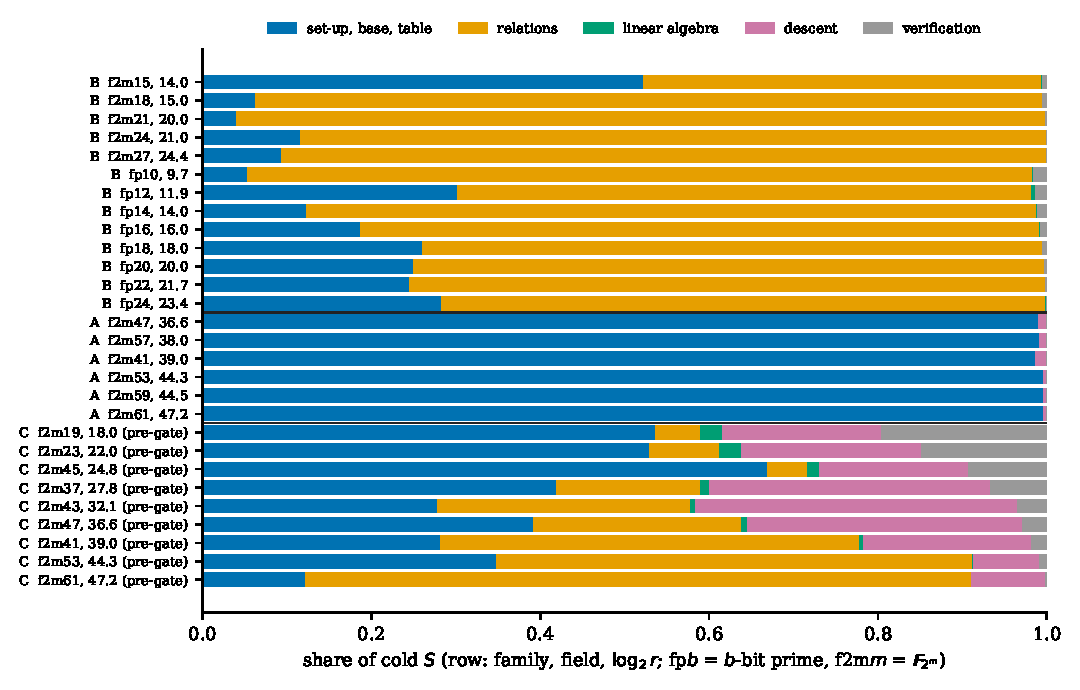
\includegraphics[width=\linewidth]{figures/fig-fm-phases.pdf}
\caption[Phase shares of cold $S$, all leaderboard rows]{Phase shares of cold $S$ for all 28 leaderboard rows, grouped
into five phases; rows marked ``pre-gate'' are unvalidated (pre-gate).
Data: \art{figures/data-fm-phases.json} (from
\art{docs/ic/leaderboard.json}); plot and shares:
\art{figures/make_fig_fm_phases.py}.}
\label{fig:fm-phases}
\end{figure}
